\documentclass[xcolor={usenames,dvipsnames},11pt]{beamer}

\defbeamertemplate{description item}{align left}{\insertdescriptionitem\hfill}

% \usetheme[sectionpage=none,subsectionpage=simple,progressbar=none,block=fill]{metropolis}
\usetheme[sectionpage=none,subsectionpage=simple,progressbar=frametitle,block=fill]{metropolis}
% \setsansfont[BoldFont={Fira Sans SemiBold}]{Fira Sans Book}
\usepackage{tikz}
\usetikzlibrary{patterns}
\usetikzlibrary{shapes.misc, positioning}
\usepackage{eso-pic}
\usepackage{booktabs}
\usepackage[scale=2]{ccicons}
\usepackage{pgfplots}
\usepackage{amsmath}
\usepackage{wasysym}
\usepackage{mathtools}
\usepackage{pgf}
\usepackage{pifont}
\usepackage{algpseudocode}
\usepackage{listings}
% \setsansfont{Ubuntu}
% \setmonofont{Ubuntu Mono}

\DeclarePairedDelimiter{\ceil}{\lceil}{\rceil}
\usepgfplotslibrary{dateplot}
\hypersetup{colorlinks,linkcolor=Cerulean,urlcolor=Cyan}

\usepackage{xspace}
\newcommand{\themename}{\textbf{\textsc{metropolis}}\xspace}
\usefonttheme[onlymath]{serif}
\setbeamertemplate{caption}{\raggedright\insertcaption\par}

\usepackage{tikz,pgfplots,filecontents}
\pgfplotsset{compat=1.7} 
\usepgfplotslibrary{colorbrewer}

\title{ \Large Turbo Codes for Deep Space Communications: CCSDS 131.0-B-2 standard implementation}
% \title{\LARGE Reccomendation for Space Data System Standards}
% \title{\Large Metropolis}
\subtitle{Final project for the Channel Coding course}
\author[G. Marcon]{Gianluca Marcon \hfill \href{mailto:gianluca.marcon.1@studenti.unipd.it}{gianluca.marcon.1@studenti.unipd.it}}
\date{\today}
\institute{University of Padova}
% \institute{Department of Information Engineering, University of Padova}

% logo on every page
%\newcommand{\nologo}{\setbeamertemplate{logo}{}}

%\newcommand\AtPagemyUpperLeft[1]{\AtPageLowerLeft{%
%\put(\LenToUnit{0.94\paperwidth},\LenToUnit{0.03\paperheight}){#1}}}
%\AddToShipoutPictureFG{
%  \AtPagemyUpperLeft{{
\includegraphics[height=2cm,keepaspectratio]{./logos/DEI.png}}}
%}%

\logo{\vspace*{-1.4cm}
\includegraphics[height=2cm,keepaspectratio]{./logos/DEI.png}}


% full logo on title page
\titlegraphic{
\includegraphics[height=2cm]{./logos/unipd}\hfill
\includegraphics[height=2cm]{./logos/DEI_full}}
\setbeamertemplate{subsection page}[simple]

\begin{document}

\maketitle

%======================================================================================
\section{Introduction}
\begin{frame}{Standard specifications}
    The standard specifies different input packet lengths $k$
    \begin{itemize}
        \item $1784$
        \item $3568$
        \item $7136$
        \item $8920$
    \end{itemize}

    ...and different code rates $R$
    \begin{itemize}
        \item $1/2$
        \item $1/3$
        \item $1/4$
        \item $1/6$
    \end{itemize}    
\end{frame}
%======================================================================================
\begin{frame}{Encoder structure}
    \begin{center}
        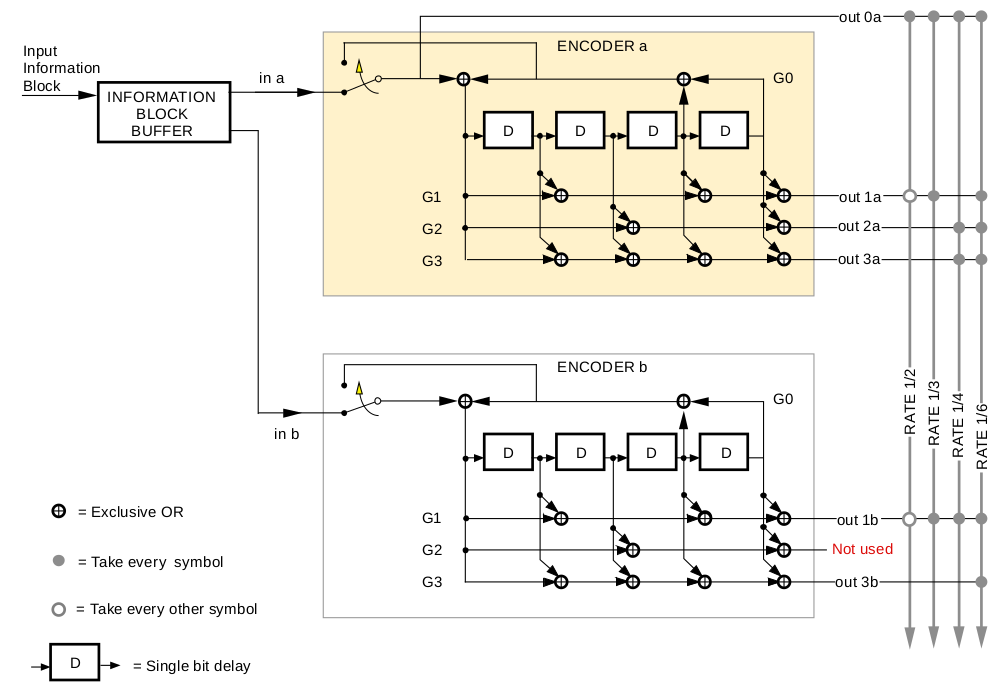
\includegraphics[height=0.75\textheight]{./images/encoder-structure}
    \end{center}
    Convolutional codes defined through forward and backward connection vectors
\end{frame}

%======================================================================================
\begin{frame}[c,fragile]{Example: defining a code in C}
    \begin{lstlisting}[
        language=C,
        basicstyle=\scriptsize,
        commentstyle=\color{mLightGreen},
        stringstyle=\color{mLightRed}
        ]
    // define first code
    int N_components = 2;
    char *forward[N_components];
    forward[0] = "10011";
    forward[1] = "10101";

    char *backward = "0011";

    t_convcode code = convcode_initialize(forward, backward, 
                                            N_components);

    t_turbocode turbo = turbo_initialize(code, code, pi,
                                            info_length);
    \end{lstlisting}
    
\end{frame}
%======================================================================================
\begin{frame}{Interleaver}
    \begin{center}
        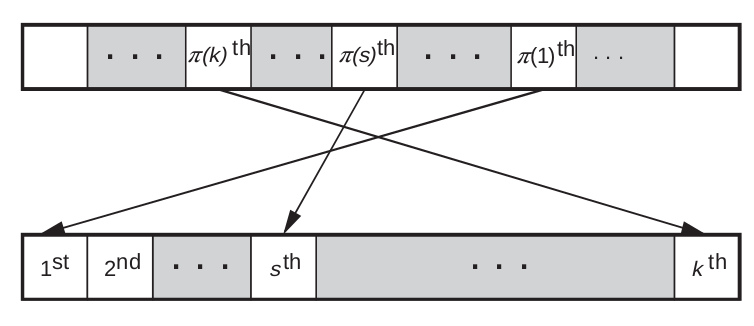
\includegraphics[width=0.5\textwidth]{./images/interleaver}
    \end{center}
    
    $i$-th bit of the interleaved packet is the $\pi(i)$-th bit of the original packet

    \begin{table}
        \centering
        \begin{tabular}{cc}
            \toprule
            Input length $k$ & $k_1 \times k_2 \times k_3$\\
            \midrule
            $1784$    &   $8  \times 223 \times 1$\\
            $3568$    &   $8  \times 223 \times 2$\\
            $7136$    &   $8  \times 223 \times 4$\\
            $8920$    &   $8  \times 223 \times 5$\\
            \bottomrule
        \end{tabular}
    \end{table}
\end{frame}

%======================================================================================
\begin{frame}{Building the interleaver}
    \begin{algorithmic}
        \State $p = \begin{bmatrix}31 & 37 & 43 & 47 & 53 & 59 & 61 & 67\end{bmatrix}$
        \For{$s = 1$ to $k$}
            \State $m = (s-1) \mod 2$
            \State $i = \text{floor}\left[(s-1)/(2k_2)\right]$
            \State $j = \text{floor}\left[(s-1)/2\right] -i k_2$
            \State $t = (19i + 1) \mod (k_1/2)$
            \State $q = t \mod 8 + 1$
            \State $c = (p_q j + 21m) \mod k_2$
            \State $\pi(s) = 2(t + c k_1/2 +1) - m$
        \EndFor
    \end{algorithmic}
\end{frame}

%======================================================================================
\begin{frame}[c]{Decoding}
    \begin{center}
        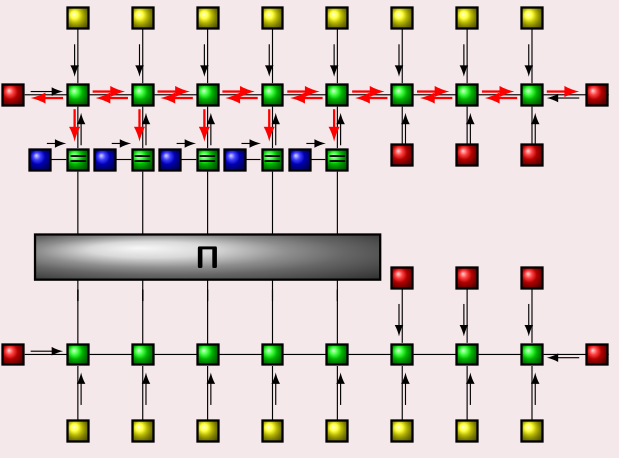
\includegraphics[width=0.5\textwidth]{./images/decoding.png}
    \end{center}
    \begin{itemize}
        \item BCJR (in log domain) on upper and lower code
        \item puncturing is applied at reception 
            $\hat{r}[i] = r[i]\cdot p[i]$ so that
            \[
                g_l(\mathbf{y}_l) \propto \exp\left( -\frac{\Vert \mathcal{L}(\mathbf{y}_l)\Vert^2}{2\sigma_w^2} \right) = \text{const}
            \]
    \end{itemize}
    
\end{frame}
%======================================================================================
\begin{frame}[c,fragile]{Example: defining a code in C}
    \begin{lstlisting}[
        language=C,
        basicstyle=\scriptsize,
        commentstyle=\color{mLightGreen},
        stringstyle=\color{mLightRed}
        ]
        // **messages is initialized to log(0.5)
        int *decoded = NULL;
        for (int i = 0; i < iterations; i++) {

            // run BCJR on upper code
            convcode_extrinsic(streams[0], lengths[0], 
                                 &messages, code.upper_code,
                                 noise_variance, 0);
            // apply interleaver
            message_interleave(&messages, code);

            // run BCJR on lower code
            // save extrinsic messages in **messages
            decoded = convcode_extrinsic(streams[1], lengths[1], 
                                 &messages, code.lower_code, 
                                 noise_variance, 
                                 i == (iterations - 1));
            // deinterleave
            message_deinterleave(&messages, code);
        }
    \end{lstlisting}
\end{frame}
%======================================================================================
% \begin{frame}[c]{Simulator options}
%     \begin{figure}
%         \centering
%        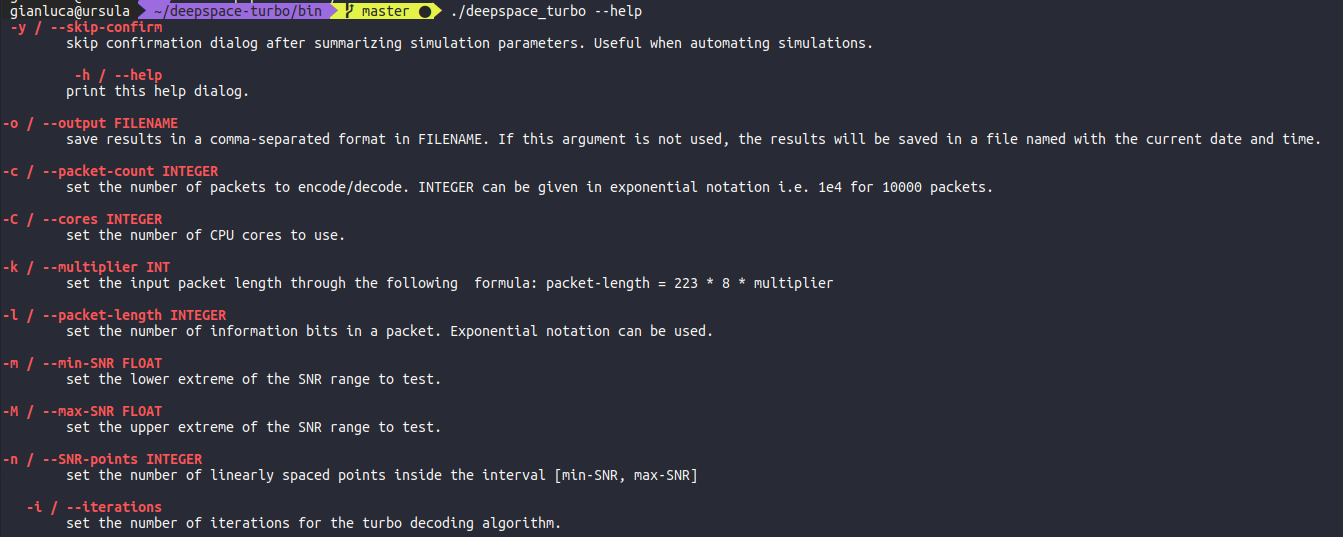
\includegraphics[width=1\textwidth]{./images/terminal}
%     \end{figure}
% \end{frame}
%======================================================================================
\begin{frame}[c]{Number of MP iterations}
    \begin{center}
        \begin{tikzpicture}
\pgfplotsset{cycle list/Set1-7,
    cycle multiindex* list={
        mark list*\nextlist
        Set1-7\nextlist
    },}

    \begin{axis}[
        clip mode=individual,
        ymode=log,
        height=0.8\textheight,
        width=0.7\textwidth,
        %every minor grid/.style={densely dotted, opacity=0.9},
        xlabel={$E_b/N_0$ [dB]},
        ylabel={BER},
        axis y line = left,
        axis x line = top,
        y axis line style = {stealth-},
        x axis line style={shorten >=-10pt},
        y axis line style={shorten <=-10pt},
        grid=both,
        xtick align=inside,
        ytick align=inside,
        xtick={0,1,...,10},
        ytick={1e-8,1e-7,1e-6,1e-5,1e-4,1e-3,1e-2,1e-1},
        line join=bevel,
        ymax = 1,
        ymin = 1e-8,
        xmax = 8,
        minor x tick num=0,
        legend style={draw=none,at={(0.5,-0.1)}, anchor=north,/tikz/every even column/.append style={column sep=5pt}},
        legend cell align=left,
        legend columns=3,
        %cycle multi list={Set1-4}
        ]
        \addplot+[
            thick,
        ] table[x=EbN0,y=BER,col sep=comma] {data/iterations/20000pkts_1iter.csv};
        \addlegendentry{1 iteration};
        
        \addplot+[
            thick,
        ] table[x=EbN0,y=BER,col sep=comma] {data/iterations/20000pkts_2iter.csv};
        \addlegendentry{2 iterations};
        
        \addplot+[
            thick,
        ] table[x=EbN0,y=BER,col sep=comma] {data/iterations/20000pkts_3iter.csv};
        \addlegendentry{3 iterations};
        
        \addplot+[
        thick,
        ] table[x=EbN0,y=BER,col sep=comma] {data/iterations/20000pkts_5iter.csv};
        \addlegendentry{5 iterations};
                    
        \addplot+[
        thick,
        ] table[x=EbN0,y=BER,col sep=comma] {data/iterations/20000pkts_7iter.csv};
        \addlegendentry{7 iterations};
        
        \addplot+[
            mark=none,
            color=black,
            style=solid,
            thick
        ] table[x=EbN0,y=BER,col sep=comma] {data/uncoded.csv};
        \addlegendentry{Uncoded};
        
        
%            \addplot+[
%            %error bars/.cd,
%            %y dir=both,
%            %y explicit,
%            %every nth mark=2
%            ] table[x=SNR,y=BER, col sep=comma] {10000pkts_2iter.csv};
%            \addlegendentry{2 iterations};
%            
%            \addplot+[
%            %error bars/.cd,
%            %y dir=both,
%            %y explicit,
%            %every nth mark=2
%            ] table[x=SNR,y=BER, col sep=comma] {10000pkts_3iter.csv};
%            \addlegendentry{3 iterations};
%
%            \addplot+[
%            %error bars/.cd,
%            %y dir=both,
%            %y explicit,
%            %every nth mark=2
%            ] table[x=SNR,y=BER, col sep=comma] {10000pkts_5iter.csv};
%            \addlegendentry{5 iterations};

    \end{axis}
\end{tikzpicture} 

    \end{center}
\end{frame}
%======================================================================================
\begin{frame}[c]{Different packet sizes: $R=1/2$}
    \begin{center}
        \begin{tikzpicture}
\pgfplotsset{cycle list/Set1-7,
    cycle multiindex* list={
        mark list*\nextlist
        Set1-7\nextlist
    },}

    \begin{axis}[
        clip mode=individual,
        ymode=log,
        height=0.8\textheight,
        width=0.7\textwidth,
        %every minor grid/.style={densely dotted, opacity=0.9},
        xlabel={$E_b/N_0$ [dB]},
        ylabel={BER},
        axis y line = left,
        axis x line = top,
        y axis line style = {stealth-},
        x axis line style={shorten >=-10pt},
        y axis line style={shorten <=-10pt},
        grid=both,
        xtick align=inside,
        ytick align=inside,
        xtick={0,1,...,10},
        ytick={1e-8,1e-7,1e-6,1e-5,1e-4,1e-3,1e-2,1e-1},
        line join=bevel,
        ymax = 1,
        ymin = 1e-8,
        xmax = 8,
        minor x tick num=0,
        legend style={draw=none,at={(0.5,-0.1)}, anchor=north,/tikz/every even column/.append style={column sep=5pt}},
        legend cell align=left,
        legend columns=3,
        %cycle multi list={Set1-4}
        ]
        \addplot+[
            thick,
        ] table[x=EbN0,y=BER,col sep=comma] {data/pktlength_rateonehalf/10000pkts_1octets.csv};
        \addlegendentry{$L=1784$};
        
        \addplot+[
            thick,
        ] table[x=EbN0,y=BER,col sep=comma] {data/pktlength_rateonehalf/10000pkts_2octets.csv};
        \addlegendentry{$L=3568$};
        
        \addplot+[
            thick,
        ] table[x=EbN0,y=BER,col sep=comma] {data/pktlength_rateonehalf/10000pkts_4octets.csv};
        \addlegendentry{$L=7136$};
        
        \addplot+[
        thick,
        ] table[x=EbN0,y=BER,col sep=comma] {data/pktlength_rateonehalf/10000pkts_5octets.csv};
        \addlegendentry{$L=8920$};
                    
        
        \addplot+[
            mark=none,
            color=black,
            style=solid,
            thick
        ] table[x=EbN0,y=BER,col sep=comma] {data/uncoded.csv};
        \addlegendentry{Uncoded};
        
        
%            \addplot+[
%            %error bars/.cd,
%            %y dir=both,
%            %y explicit,
%            %every nth mark=2
%            ] table[x=SNR,y=BER, col sep=comma] {10000pkts_2iter.csv};
%            \addlegendentry{2 iterations};
%            
%            \addplot+[
%            %error bars/.cd,
%            %y dir=both,
%            %y explicit,
%            %every nth mark=2
%            ] table[x=SNR,y=BER, col sep=comma] {10000pkts_3iter.csv};
%            \addlegendentry{3 iterations};
%
%            \addplot+[
%            %error bars/.cd,
%            %y dir=both,
%            %y explicit,
%            %every nth mark=2
%            ] table[x=SNR,y=BER, col sep=comma] {10000pkts_5iter.csv};
%            \addlegendentry{5 iterations};

\end{axis}
\end{tikzpicture}

    \end{center}
\end{frame}
%======================================================================================
\begin{frame}[c]{Different packet sizes: $R=1/4$}
    \begin{center}
        \begin{tikzpicture}
\pgfplotsset{cycle list/Set1-7,
    cycle multiindex* list={
        mark list*\nextlist
        Set1-7\nextlist
    },}

    \begin{axis}[
        clip mode=individual,
        ymode=log,
        height=0.8\textheight,
        width=0.7\textwidth,
        %every minor grid/.style={densely dotted, opacity=0.9},
        xlabel={$E_b/N_0$ [dB]},
        ylabel={BER},
        axis y line = left,
        axis x line = top,
        y axis line style = {stealth-},
        x axis line style={shorten >=-10pt},
        y axis line style={shorten <=-10pt},
        grid=both,
        xtick align=inside,
        ytick align=inside,
        xtick={0,1,...,10},
        ytick={1e-8,1e-7,1e-6,1e-5,1e-4,1e-3,1e-2,1e-1},
        line join=bevel,
        ymax = 1,
        ymin = 1e-8,
        xmax = 8,
        minor x tick num=0,
        legend style={draw=none,at={(0.5,-0.1)}, anchor=north,/tikz/every even column/.append style={column sep=5pt}},
        legend cell align=left,
        legend columns=3,
        %cycle multi list={Set1-4}
        ]
        \addplot+[
            thick,
        ] table[x=EbN0,y=BER,col sep=comma] {data/pktlength_rateonefourth/10000pkts_1octets.csv};
        \addlegendentry{$L=1784$};
        
        \addplot+[
            thick,
        ] table[x=EbN0,y=BER,col sep=comma] {data/pktlength_rateonefourth/10000pkts_2octets.csv};
        \addlegendentry{$L=3568$};
        
        \addplot+[
            thick,
        ] table[x=EbN0,y=BER,col sep=comma] {data/pktlength_rateonefourth/10000pkts_4octets.csv};
        \addlegendentry{$L=7136$};
        
        \addplot+[
        thick,
        ] table[x=EbN0,y=BER,col sep=comma] {data/pktlength_rateonefourth/10000pkts_5octets.csv};
        \addlegendentry{$L=8920$};
                    
        
        \addplot+[
            mark=none,
            color=black,
            style=solid,
            thick
        ] table[x=EbN0,y=BER,col sep=comma] {data/uncoded.csv};
        \addlegendentry{Uncoded};
        
\end{axis}
\end{tikzpicture}

    \end{center}
\end{frame}
%======================================================================================
\begin{frame}[c]{Codes comparison: $L=8920$}
    \begin{center}
        \begin{tikzpicture}
\pgfplotsset{cycle list/Set1-7,
    cycle multiindex* list={
        mark list*\nextlist
        Set1-7\nextlist
    },}

    \begin{axis}[
        clip mode=individual,
        ymode=log,
        height=0.8\textheight,
        width=0.7\textwidth,
        %every minor grid/.style={densely dotted, opacity=0.9},
        xlabel={$E_b/N_0$ [dB]},
        ylabel={BER},
        axis y line = left,
        axis x line = top,
        y axis line style = {stealth-},
        x axis line style={shorten >=-10pt},
        y axis line style={shorten <=-10pt},
        grid=both,
        xtick align=inside,
        ytick align=inside,
        xtick={0,1,...,10},
        ytick={1e-8,1e-7,1e-6,1e-5,1e-4,1e-3,1e-2,1e-1},
        line join=bevel,
        ymax = 1,
        ymin = 1e-8,
        xmax = 8,
        minor x tick num=0,
        legend style={draw=none,at={(0.5,-0.1)}, anchor=north,/tikz/every even column/.append style={column sep=5pt}},
        legend cell align=left,
        legend columns=3,
        %cycle multi list={Set1-4}
        ]
        \addplot+[
            thick,
        ] table[x=EbN0,y=BER,col sep=comma] {data/rate_4octets/10000pkts_code1.csv};
        \addlegendentry{$R=1/2$};
        
        \addplot+[
            thick,
        ] table[x=EbN0,y=BER,col sep=comma] {data/rate_4octets/10000pkts_code2.csv};
        \addlegendentry{$R=1/3$};
        
        \addplot+[
            thick,
        ] table[x=EbN0,y=BER,col sep=comma] {data/rate_4octets/10000pkts_code3.csv};
        \addlegendentry{$R=1/4$};
        
        \addplot+[
        thick,
        ] table[x=EbN0,y=BER,col sep=comma] {data/rate_4octets/10000pkts_code4.csv};
        \addlegendentry{$R=1/6$};
                    
        
        \addplot+[
            mark=none,
            color=black,
            style=solid,
            thick
        ] table[x=EbN0,y=BER,col sep=comma] {data/uncoded.csv};
        \addlegendentry{Uncoded};
        
\end{axis}
\end{tikzpicture}

    \end{center}
\end{frame}
%======================================================================================
\begin{frame}[c]{Codes comparison: a closer look}
    \begin{center}
        \begin{tikzpicture}
\pgfplotsset{cycle list/Set1-7,
    cycle multiindex* list={
        mark list*\nextlist
        Set1-7\nextlist
    },}

    \begin{axis}[
        clip mode=individual,
        ymode=log,
        height=0.8\textheight,
        width=0.7\textwidth,
        %every minor grid/.style={densely dotted, opacity=0.9},
        xlabel={$E_b/N_0$ [dB]},
        ylabel={BER},
        axis y line = left,
        axis x line = top,
        y axis line style = {stealth-},
        x axis line style={shorten >=-10pt},
        y axis line style={shorten <=-10pt},
        grid=both,
        xtick align=inside,
        ytick align=inside,
        xtick={0,0.5,1,1.5,2},
        ytick={1e-8,1e-7,1e-6,1e-5,1e-4,1e-3,1e-2,1e-1},
        line join=bevel,
        ymax = 1,
        ymin = 1e-8,
        xmax = 2,
        minor x tick num=1,
        legend style={draw=none,at={(0.5,-0.1)}, anchor=north,/tikz/every even column/.append style={column sep=5pt}},
        legend cell align=left,
        legend columns=3,
        %cycle multi list={Set1-4}
        ]
        \addplot+[
            thick,
        ] table[x=EbN0,y=BER,col sep=comma] {data/rate_4octets/10000pkts_code1.csv};
        \addlegendentry{$R=1/2$};
        
        \addplot+[
            thick,
        ] table[x=EbN0,y=BER,col sep=comma] {data/rate_4octets/10000pkts_code2.csv};
        \addlegendentry{$R=1/3$};
        
        \addplot+[
            thick,
        ] table[x=EbN0,y=BER,col sep=comma] {data/rate_4octets/10000pkts_code3.csv};
        \addlegendentry{$R=1/4$};
        
        \addplot+[
        thick,
        ] table[x=EbN0,y=BER,col sep=comma] {data/rate_4octets/10000pkts_code4.csv};
        \addlegendentry{$R=1/6$};
                    
        
        \addplot+[
            mark=none,
            color=black,
            style=solid,
            thick
        ] table[x=EbN0,y=BER,col sep=comma] {data/uncoded.csv};
        \addlegendentry{Uncoded};
        
\end{axis}
\end{tikzpicture}

    \end{center}
\end{frame}
%======================================================================================
\begin{frame}[standout]

    \begin{center}
        Source code for simulator, scripts, plotting and presentation available at \\ \url{http://github.com/geeanlooca/deepspace-turbo}
    \end{center}


    {
        \huge Thank you!
    }
\end{frame}
% %======================================================================================

\end{document}
